

%%%%%%%%%%%%%%%%%%%%%%%%%%%%%%%%%%%%%%%%%%%%%%%%%%%%%%%%%%%%%%%%%%%%%%%%%%%%%%%%%%%%%%%%%%%%%%%%
% Carbon
%%%%%%%%%%%%%%%%%%%%%%%%%%%%%%%%%%%%%%%%%%%%%%%%%%%%%%%%%%%%%%%%%%%%%%%%%%%%%%%%%%%%%%%%%%%%%%%%

\chapter{FLR impacts on climate change mitigation} \label{ch:carbon}


Current net carbon emissions due to tropical deforestation and degradation are estimated to contribute to 8-15 \% (approx. 1.1 GtC) of the total global anthropogenic carbon emissions \citep{Houghton2015ACO2, Brinck2017HighCycle}. Deforestation contributes to CO2 emissions by burning the vegetation biomass and releasing carbon from soils \citep{Wang2016DynamicsChina}. Concerns regarding global climate change have motivated policymakers from many countries to implement regulations and policies aiming to minimize national emissions of carbon dioxide \citep{Stavins1997PolicyProblem, Clarkson2015TheScheme}. Historically, efforts have been directed mainly to preventing deforestation and degradation of tropical forests, but FLR can play an important role in mitigating climate change \citep{Chazdon2016c,Locatelli2015TropicalCarbon}. 

Tropical forest restoration can sequester large amounts of carbon from the atmosphere into the above and below-ground biomass (AGB) and into the soil \citep{Silver2000TheLands, Lal2004SoilSecurity, Cunningham2015BalancingRegions}. Neotropical secondary forests, for example, accumulate biomass at a rate 11\% higher than mature forests \citep{Poorter2016}. If all secondary forest currently occurring in the Neotropics is allowed to grow, it can potentially sequester a total of 31.09 Pg CO2 in the next 40 years, which is equivalent to carbon emissions from fossil fuel use and industrial processes in all of Latin America and the Caribbean from 1993 to 2014 \citep{Chazdon2016c}. Another study estimates that restoring 500 million hectares of tropical forests could sequester approximately 1 PgC yr−1 \citep{Houghton2015ACO2}. Although most studies focus on carbon sequestration by the above-ground biomass, vegetation regrowth dynamics and associated biomass decomposition increase organic carbon concentration in the soil forming a stable carbon storage \citep{Xu2018EffectsChina}. 

	Studies have shown that forest restoration can increase C stocks in the soil through the addition of organic carbon from the decomposition of trunks, litter and roots (e.g. \citep{Macedo2008ChangesTrees, RodriguesNogueiraJr.2011SoilSpecies, Xu2018EffectsChina}. Soils can potentially accumulate carbon at a rate of 1.30 Mg ha-1 yr-1 during the first 20 years of forest establishment and at a rate of 0.20 Mg ha-1 yr-1 in the subsequent 80 years \citep{Silver2000TheLands}. Estimates on the potential C sequestration by world soils vary widely, ranging from 0.4 GtC yr -1 to 1.2 GtC yr-1 \citep{Sauerbeck2001CO2emissionsLimitations, Lal2004SoilSecurity}. Such uncertainty is partly related to the fact that the dynamics of carbon cycling in the soil during forest regrowth, particularly in the tropics, is still poorly understood \citep{Ritchie2014PlantGrassland, Wang2016DynamicsChina, Xu2018EffectsChina}. Additionally, past land-use history, restoration age and restoration method (active, natural regeneration or agroforestry systems) are important factors determining the rates of biomass and soil carbon accumulation during tropical forest regeneration. Therefore, there is a need to investigate how efficient different restoration methods can be in different landscape contexts. 


%---------------------------------------------------------------------------------------------
\section{\Large Soil quality indicators for FLR in the Atlantic Forest}  \label{sec:car-air}

Consideration of soil quality indicators is crucial for planning the management and restoration of ecosystems. We conducted a systematic literature review to understand how restoration initiatives in the Atlantic Forest have accounted for soil indicators in their planning and management decisions \citep{Mendes2018}. From the 152 retrieved studies, only 41\% (62) reported any soil data. Among those, only 40\% of the retrieved studies included information on soil conditions before the restoration took place (project baseline) or from reference sites. Out of the studies that had reference sites (N =25), the most cited soil indicators were Phosphorus and pH (56\%, N=14) followed by carbon (52\%; N=13), potassium (48\%; N =12), nitrogen (44\%; N =11), aluminium (31\%; N =8), edaphic fauna (20\%;N =5), CEC (16\%; N =4), and iron (12\%; N =3). It was surprising that soil organic matter, a fundamental indicator for ecosystem services such as carbon sequestration, was rarely evaluated. 

The results of this work demonstrate a soil data gap within the restoration projects in the Brazilian Atlantic Forest. Moreover, we observed that even if a study includes information about soil properties, such information is frequently added “bureaucratically” without appropriate contextualization or evaluation of observed patterns. Such lack of information impedes an accurate analysis on management needs and on the efficiency of restoration techniques for soil and ecosystem restoration. We conclude that despite the evidence regarding the importance of soil for the provision of global and local ecosystem services, soil remains an under-investigated aspect of the environment. This published work calls attention of scientists and practitioners to include basic soil analysis in their studies and monitoring in order to maximize the successful outcomes of restoration. In a follow up study, still ongoing, we are further investigating the effect size of the most cited soil properties to restoration activities. We have included only studies that present a reference site and will calculate the response ratios (which is calculated as the ratio between the restored area and the reference) in order to identify how fast the different soil indicators are restored and which factors might affect restoration efficiency. Among the factors being evaluated are soil type, restoration age and previous land-use history.  


%---------------------------------------------------------------------------------------------

\section{\Large FLR impacts on carbon stocks in the Amazon and Atlantic Forest}  \label{sec:car-soil}

Ecological restoration of forest ecosystems is expected to contribute to climate change mitigation through carbon sequestration in the above and below ground biomass and in the soils. The efficiency of a restored area to store carbon in the different compartments, however, may depend on the context of degradation and on the restoration technique applied. 

To summarize the current knowledge on the impacts of FLR on climate change mitigation, we have conducted a literature review on studies from all Brazilian biomes, with special focus on the Amazon and Atlantic Forest (see methodology in section \ref{subsec:bio-revisão}). Among the selected studies, 78 measured carbon stocks in the soil (49, 63\%) or in the plant (26 studies, 33\%) and animal biomass (3, 4\%) (Figure \ref{fig:Carb-Cata-1} A). In the forest biomes 67 studies were selected, with the majority being in the Atlantic Forest (52 studies, 78\%) (Figure \ref{fig:Carb-Cata-1} B). Interestingly most studies analyzed soil carbon and not vegetation biomass. A possible reason for this unexpected result is that studies on plant biomass in secondary forests or active restorations do not have a reference ecosystem but make comparisons to reference values from other published work. Soil studies, on the other hand, may more often take measures of a reference ecosystem due to the large heterogeneity in soils which may hamper comparisons to other studies. We will further investigate such reasons in our dataset. Nevertheless, the high availability of data on soils may allow us to perform accurate statistical analyses and identify how different restoration techniques and land use histories affect the capacity of restored systems to recover soil carbon stocks. 

This will contribute to fill up the gap on how efficient the management techniques have been in restoring soil carbon stocks in forest ecosystems of Brazil (see section \ref{sec:car-air}). Additionally, a subset of studies provided information on both biodiversity and carbon stocks (21 studies for both biomes), which will allow us to test if there is a correlation between biodiversity and carbon stocks restoration. 


 %%%%%% FIgura Carb-Cata-1 %%%%%%%% 
\begin{figure}[H]
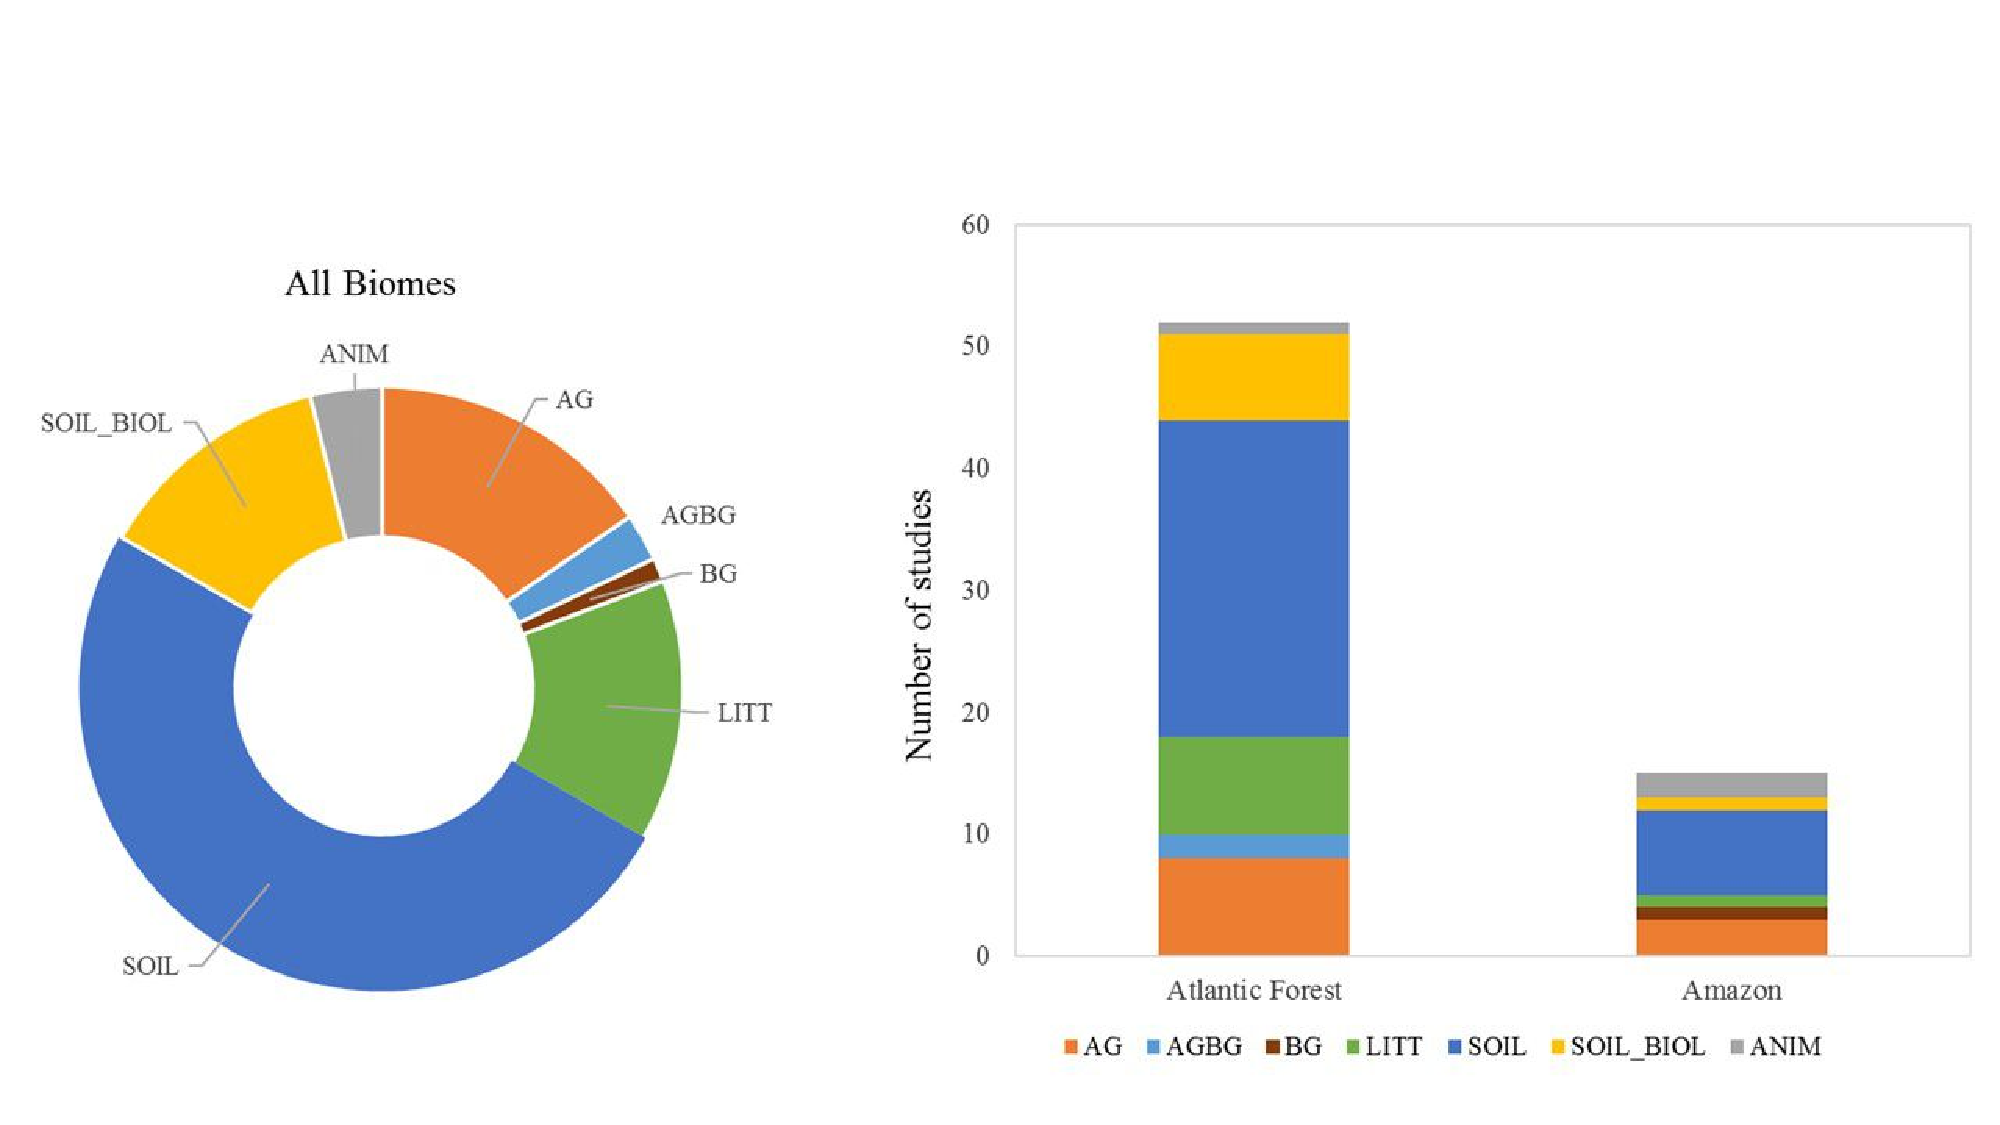
\includegraphics[width=1.0\linewidth]{pictureve/Carb-Cata-1.pdf}
\caption{(A) Proportion of studies on the effects of restoration on carbon stocks in the different compartments and (B) number of studies in the Brazilian Atlantic Forest and Amazon biomes that evaluated restoration effects on the carbon stocks in the: aboveground biomass (AG), belowground biomass (BG), above and belowground biomass together (AGBG), litter biomass (LITT), soil (SOIL), microflora and fauna biomass of the soil (SOIL-BIOL) and animal biomass (ANIM).}
\label{fig:Carb-Cata-1}
\end{figure}

%\textcolor{blue}{Figure Carb-Cata-1.  (A) Proportion of studies on the effects of restoration on carbon stocks in the different compartments and (B) number of studies in the Brazilian Atlantic Forest and Amazon biomes that evaluated restoration effects on the carbon stocks in the: aboveground biomass (AG), belowground biomass (BG), above and belowground biomass together (AGBG), litter biomass (LITT), soil (SOIL), microflora and fauna biomass of the soil (SOIL-BIOL) and animal biomass (ANIM).} 



%---------------------------------------------------------------------------------------------

\section{\Large Mapping the potential carbon sequestration by FLR in Brazil}  \label{sec:car-soil}

Brazil large area of forests and high deforestation rates makes it a critical player to any global scenario of carbon emission. On the other hand, large extents of Brazilian land are expected to be restored to its native vegetation under PLANAVEG \citep{BrazilianMinistryofEnvironment2017}. Quantifying the potential carbon sequestration to be promoted by restoration is crucial to recognize the role of FLR in mitigating climate change and to support public policies. 

Aiming to provide such estimate at the national level, we are currently developing the first map of potential carbon sequestration by above-ground biomass restoration in the six Brazilian biomes. To achieve this goal, we are building a predictive model of above-ground carbon stocks based on carbon stocks in native mature vegetation as a function of a set of environmental variables (soil properties, climatic variables, elevation, etc.) and past disturbance descriptors (frequency of fire, intensity of previous land use). 

We are using carbon estimates of native forest vegetation provided by \cite{Englund2017}, which had the most updated current-land-use carbon map for Brazil (50 m). This map has important advantages over the remote sensing estimates like Saatchi \cite{SaatchiSSHarrisNLBrownSLefskyMMitchardETSalasWZuttaBRBuermannWLewisSLHagenSPetrovaSWhiteLSilmanM2011BenchmarkContinents}  and Baccini \cite{Baccini2012}: (i) it provides more accurate carbon values for agricultural and pastures lands and for non-forest ecosystems, (ii) it extends over the subtropics, which hold portions of the Atlantic forest biome, (iii) is based on the most recent land cover map for Brazil \citep{Sparovek2015}. We are restricting our sampling to areas that are knowingly covered by native vegetation and have been little disturbed, which required a massive effort to compile georeferenced data from ecological studies and vegetation inventories where the authors describe the vegetation type and some information on disturbance history (in total we have compiled ~6,200 points). We have already compiled the best available spatially explicit information on all predictor variables to be used in the modelling, being 8 disturbance descriptors (based on Dias \cite{Dias2016a}, INPE), 2 topographic variables (USGS, INPE), 4 soil variables (SoilGrids) and 19 Bioclimatic variables (Bioclim).

We have already extracted the information from all these layers for each native vegetation sample point. The next steps will be to select the most appropriate set of predictor variables, run the regression models, and validate the models using a subsample of the original dataset. Once we have identified the relationships between carbon stocks and the most meaningful predictors, we will apply the model to the deforested areas to predict the potential carbon sequestration by forest restoration. The resulting map – the first of its kind for a country – will also be one of the layers used for the spatial prioritization of restoration. 


%\textcolor{red}{Box C. teeb carbono- Carbon sequestration was slightly higher in SS than in LC, but this difference was due not to the different strategies for allocating restoration but, instead, to the expansion of agroforestry systems in SS.MAPS}